%%%%
\documentclass[12pt, a4paper]{report}

% packages...
\usepackage[utf8]{inputenc}
\usepackage[english, italian]{babel}
\usepackage[hyphens]{url}
\usepackage{csquotes}
\usepackage{caption}
\usepackage{subcaption}
% Per generare il file PDF aderente alle specifiche PDF/A-1b. Verificarne poi la validità.
%\usepackage[a-1b]{pdfx}

\usepackage{hyperref}
\usepackage{graphicx}
\graphicspath{ {Img/} }
\usepackage{lipsum}% Per inserire testo a caso in attesa di realizzare i capitoli
\usepackage{listings}
\usepackage{epigraph} % per le frasi inizio capitolo
\usepackage{fancyhdr}
% \usepackage{refcheck}

\usepackage{pgfplots} 
%\pgfplotsset{compat=1.18} 

\usepackage{verbatim}

\lstset{
	% 	language=bash
	frame=single, 
	breaklines=true, 
	postbreak=\raisebox{0ex}[0ex][0ex]{\ensuremath{\color{red}\hookrightarrow\space}}, 
	basicstyle=\ttfamily\footnotesize
}

%MyStyle
\renewcommand{\lstlistingname}{Code}

\definecolor{codegray}{rgb}{0.5, 0.5, 0.5}
\definecolor{codepurple}{rgb}{0.58, 0, 0.82}
\definecolor{backcolour}{rgb}{0.95, 0.95, 0.92}

\lstdefinestyle{Cstyle}{
 backgroundcolor=\color{backcolour}, 
 keywordstyle=\color{blue}, 
 numberstyle=\tiny\color{codegray}, 
 stringstyle=\color{codepurple},
 basicstyle=\ttfamily\footnotesize, 
 breakatwhitespace=false, 
 breaklines=true, 
 captionpos=b, 
 keepspaces=true, 
 numbers=left, 
 numbersep=5pt, 
 showspaces=false, 
 showstringspaces=false, 
 showtabs=false, 
 tabsize=2, 
 frame = leftline
}

% RISC style
\lstdefinelanguage{Risc-v}
{
 alsoletter={.}, % allow dots in keywords
 alsodigit={0x}, % hex numbers are numbers too!
 morekeywords=[1]{ % instructions
 lb, lh, lw, lbu, lhu,
 sb, sh, sw, 
 sll, slli, srl, srli, sra, srai, 
 add, addi, sub, lui, auipc, addiw
 xor, xori, or, ori, and, andi, 
 slt,slti, sltu, sltiu, 
 beq, bne, blt, bge, bltu, bgeu, 
 j,jr, jal, jalr, ret, 
 scall, break, nop
 }, 
 morekeywords=[2]{ % sections of our code and other directives
 .align, .ascii,.asciiz, .byte,.data, .double,.extern, 
 .float, .globl, .half, .kdata, .ktext, .set, .space, .text, .word
 }, 
 morekeywords=[3]{ % registers
 zero, ra,sp, gp,tp, s0,fp, 
 t0, t1,t2, t3,t4, t5, t6, 
 s1,s2, s3, s4,s5, s6, s7,s8, s9, s10,s11, 
 a0,a1, a2, a3,a4, a5, a6, a7,
 ft0, ft1, ft2,ft3, ft4,ft5, ft6,ft7, 
 fs0, fs1,fs2, fs3, fs4,fs5, fs6, fs7,fs8, fs9, fs10,fs11, 
 fa0, fa1, fa2, fa3, fa4, fa5, fa6,fa7
 }, 
 morecomment=[l]{;}, % mark ; as line comment start
 morecomment=[l]{\#},% as well as # (even though it is unconventional)
 morestring=[b]", % mark " as string start/end
 morestring=[b]' % also mark ' as string start/end
}

\lstset{
 % listings sonderzeichen (for german weirdness)
 literate={ö}{{\"o}}1
 {ä}{{\"a}}1
 {ü}{{\"u}}1,
 basicstyle=\tiny\ttfamily, % very small code
 breaklines=true, % break long lines
 commentstyle=\itshape\color{green!50!black}, % comments are green
 keywordstyle=[1]\color{blue!80!black},% instructions are blue
 keywordstyle=[2]\color{orange!80!black}, % sections/other directives are orange
 keywordstyle=[3]\color{red!50!black}, % registers are red
 stringstyle=\color{mauve}, % strings are from the telekom
 identifierstyle=\color{teal}, % user declared addresses are teal
 frame=l, % black line on the left side of code
 language=Risc-v, % all code is RISC-V
 tabsize=4, % indent tabs with 4 spaces
 showstringspaces=false % do not replace spaces with weird underlines
}

%--- BIBIOGRAFIA
 \usepackage[ backend=biber,
sorting=ynt, 
%citestyle=authoryear 
]{biblatex}

\addbibresource{Bibliografia.bib}
%---

\usepackage[textwidth=2cm, textsize=scriptsize,colorinlistoftodos]{todonotes}
\setlength {\marginparwidth }{2cm}
%\usepackage[disable]{todonotes}

%%%%%%%%%%%%%%%%%%%%%%%%%%%%%%%%%%%%%%%%%%%%%%%%%%%%%
\begin{document}
% Frontespizio
\begin{titlepage}
\begin{center}

\includegraphics[width=\textwidth]{Img/Logo.jpg}\\
{\large{\bf Corso di Laurea Informatica}}
\end{center}
\vspace{12mm}
\begin{center}

\vspace{4mm}
{\huge{\bf RISC-V stress testing}}\\
\vspace{4mm}

\end{center}
\vspace{12mm}
\begin{flushleft}
{\large{\bf Relatore:}}
{\large{Trentini Andrea}}\\
\vspace{4mm}
{\large{\bf Correlatore:}}
{\large{Carraturo Alexjan}}\\
\end{flushleft}
\vspace{12mm}
\begin{flushright}
{\large{\bf Tesi di Laurea di:}}
{\large{Bianchessi Mattia}}\\
{\large{\bf Matr. 931455}}\\
\end{flushright}
\vspace{4mm}
\begin{center}
{\large{\bf Anno Accademico 2021-2022}}
\end{center}
\end{titlepage}


\listoftodos


\tableofcontents
\listoffigures
\listoftables
\lstlistoflistings



%%%%%%%%
\chapter{Introduzione}
%\textbf{Oggetto della tesi}
Il processore è il componente hardware con il quale vengono svolte le istruzioni.
Oggigiorno sono presenti numerosi processori, ognuno caratterizzato da un insieme di istruzioni che definiscono  cosa un processore può eseguire. RISC-V, con un \textit{istruction set} basato su un approccio \textit{reduced instruction set computer}\cite{RISCOverview}, sta facendo parlare di sè \cite{RISCVHistory}.

%\textbf{OBIETTIVI}
L'obiettivo di questa tesi è quello di fare alcuni test sul processore dotato di RISC-V e valutarne le prestazioni.

%\textbf{METODI E STRUMENTI}
Per la valutazione sono stati utilizzati due benchmark (Coremark, LINPACK) e alcuni
codici in linguaggio C compilati con la \textit{toolchain} di RISC-V.I risultati dei test vengono riportati e, in alcuni casi, comparati con i risultati di programmi simili compilati per altri processori. Viene poi analizzato il codice sorgente generato in linguaggio macchina e confrontato con altri codici generati.

%\textbf{Struttura }
La tesi inizia con una panoramica sul progetto RISC-V presentando gli obiettivi e la storia del progetto. Il secondo capitolo mostra in sintesi l'ISA di RISC-V presentando alcuni punti importanti del progetto. Successivamente con il capitolo tre vengono presentati i compilatori mostrando la storia dalle origini fino ai compilatori moderni e la cross-compilazione. In particolare viene presentata la \textit{toolchain} utilizzata per la compilazione dei programmi.
Nei capitoli quattro e cinque vengono presentati i programmi utilizzati e i risultati ottenuti vengono analizzati nel capitolo sei.


% o sections (dipende dal documentclass)
\chapter{RISC-V}
% OUTLINE CH 1 
% ->>>>Un approccio meno giornalistico 
%	1- presentazione progetto, (1.1- obbiettivi )
%	2- storia \\
RISC-V è una ISA basato sul principio RISC nato come progetto accademico. Nel 2010, a Berkeley(California), il progetto inizi\'o diretto dal prof. David Patterson finanziato da \textit{Intel } e \textit{Microsoft} e da alcune aziende Californiane. La prima pubblicazione è dell'anno successivo. Nel 2015 viene fondata \textbf{RISC-V Foudation}, un' azienda no-profit che controlla lo sviluppo di RISC-V. Nel 2018 viene annunciata una collaborazione tra l'azienda e \textit{Linux Foundation} con la quale si supporta lo sviluppo del progetto RISC-V \cite{RISCOrgHistory}.


\section{Gli obbiettivi di RISC-V}
Durante la fase di progettazione, i progettisti hanno voluto mettere nero su bianco lo scopo di RISC-V. Gli obbiettivi dichiarati nell'introduzione della specifica dell'ISA user-mode sono:
\begin{itemize}
	\item un ISA con una licenza \textit{open source} disponibile per accademia e industria.
	\item un ISA adatta ad un'implementazione hardware diretta, non una simulazione.
	\item un ISA non specifica per una micro-architettura o una tecnologia ma che permetta un implementazione efficiente.
	\item un ISA modulare,organizzata in ISA più piccole con la possibilità di usare estensioni\footnote{Insiemi di istruzioni opzionali che possono essere aggiunte alla base dell'ISA di RISC-V per fornire funzionalità specifiche. Sezione \ref{estensioni}.}.
	\item supporto per lo standard floating-point 2008 IEEE-754 \footnote{ \url{https://ieeexplore.ieee.org/document/4610935} \cite{IEEE754-2008}}.
	\item supporto delle estensioni. 
	\item spazio di indirizzamento 32 e 64 bit.
	\item supporto a delle implementazioni multi core e manycore \footnote{I processori Manycore sono un tipo speciale di processori multi-core progettati per un alto grado di elaborazione parallela. Contengono numerose core più semplici e indipendenti. } sia eterogenei che omogenei.
	\item istruzioni a lunghezza variabile.
	\item un ISA completamente virtualizzabile.
	\item un ISA che permetta la semplificazione degli esperimenti con nuovi progetti ISA con \textit{supervisor-level} e \textit{hypervisor-level}. 
	
\end{itemize}

\section{Panoramica}
L'ISA RISC-V è un architettura load-store con solo 49 istruzioni base. L'ISA supporta sistemi di memoria sia \textit{little-endian} che \textit{big-endian}. Le istruzioni sono organizzate in pacchetti da 16-bit memorizzati in maniera \textit{little-endian} indipendentemente dall'\textit{endianness} del sistema. Ogni pacchetto ha nei bit meno significativi i bit per la codifica delle istruzioni. In questo le istruzioni di lunghezza variabile sono decodificate velocemente.

Le celle della memoria principale sono di lunghezza variabile a seconda dell'ISA base scelto, il numero di celle di memoria è XLEN e la dimensione della singola cella è di $2^{XLEN - 1}$. Ad esempio l'ISA RV32I ha un XLEN di 32. Lo spazio di indirizzamento è circolare quindi l'errore di overflow non c'è in quanto i calcoli degli indirizzi vengono scalati in modo adeguato dividendosi per un modulo adatto sfruttando cosi la caratteristica circolare \cite{ISA}.


%Modalita indirizzamento
Avendo tutte le istruzioni di lunghezza fissa, non è possibile avere direttamente costanti o indirizzi superiori alla lunghezza assegnata al campo dell'istruzione. La soluzione è l'utilizzo della modalità di indirizzamento:
\begin{itemize}
	\item \textbf{indirizzamento immediato}: l’operando è una costante nell’istruzione è comunque limitato dai bit assegnati del campo.
	\item \textbf{indirizzamento a registro}: l’operando è un registro.
	\item \textbf{indirizzamento di base con spostamento}: l’operando è la somma tra il
contenuto di un registro e una costante.
\item \textbf{indirizzamento relativo al PC}: l'operando dipende dal \textit{Program Counter} che viene sommato a una costante.
\end{itemize}


%Eccezioni, trap, iterrupt
Si parla di eccezione quando una condizione non comune avviene a \textit{run time} associata a un'istruzione.
Si parla di \textit{trap} quando si verifica un trasferimento di controllo da parte del \textit{trap handler}, da un \textit{thread} ad un altro. Si parla di \textit{interrupt} quando la situazione imprevista è qualcosa di esterno.



\section{Descrizione board} 

La scheda di sviluppo utilizzata è D1-H Nezha basata sul design del chip Allwinner D1-H. La board integra una CPU Ali Pingtou Ge RISC-V C906, con clock a 1 GHz, supporta il kernel Linux standard, ha la memoria 2G DDR3, 258 MB di spin-nand, connessione WiFi/Bluetooth, con interfacce audio e video, può essere collegata a varie periferiche, MIPI-DSI+TP, supporta il collegamento con scheda SD, HDMI, auricolari da 3,5 mm, Gigabit Ethernet, USB,USB-C, UART, 40 pin.


\begin{figure}[!ht]
\includegraphics[width = \textwidth]{D1H-BoardTopView.png}
\caption{Board vista dall'alto}

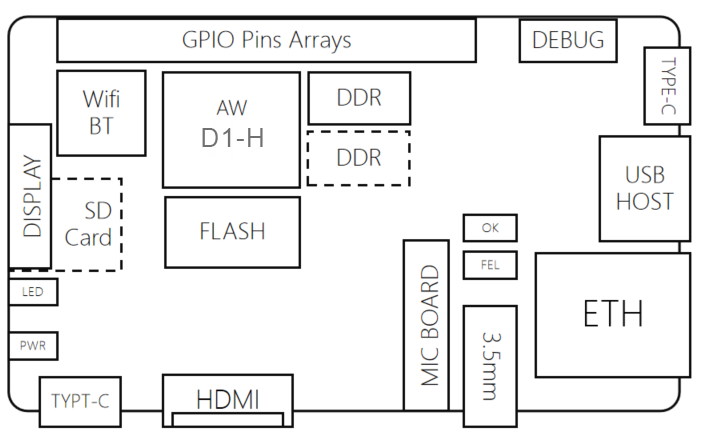
\includegraphics[width = \textwidth]{D1H-BoardBlockView.png}
\caption{Schema a blocchi della scheda di sviluppo}\cite{BoardInfo}
\end{figure}

\vspace{2cm}

\begin{table}[!ht]
\centering
\begin{tabular}{| r | c |}
\hline
CPU & Allwinner D1-H \\
\hline
Clock & 1GHz\\
\hline
DRAM & DDR3 2GB\\
\hline
Memoria & 256MB spin-nand integrato\\
\hline 
Supporto memoria & USB e SD\\
\hline
Rete & Gigabit Ethernet, 2.4G WiFi e Bluetooth, antenna integrata\\
\hline
Display & MIPI-DSI + TP, HDMI,SPI \\
\hline
Audio & jack per cuffie da 3,5 mm\\
\hline
Tasti & FEL, LRADC OK\\
\hline
Luci & alimentazione, LED tricolore\\
\hline
DEBUG & UART, USB ADB\\
\hline
USB & USB, USB OTG, USB2.0\\
\hline
PIN & array di pin 40\\
\hline
Alimentazione & USB-C 5V-2A\\
\hline
Dimensioni & 85 x 56 x 1,7 mm\\
\hline

\end{tabular}
\caption{Caratteristiche della board}
\end{table}

\section{Ambiente di sviluppo}
La scheda di sviluppo D1-H viene fornita con il sistema Tina Linux. Il kernel fornito \'e adattato al kernel Linux 5.4. La board fornisce il supporto di base e gestione delle risorse hardware del dispositivo. Ulteriori informazioni sono disponibili sul sito della board
\footnote{Link al sito della board in esame \url{https://d1.docs.aw-ol.com/study/study_1tina/}}.


%%
% Capitolo 2
% BASE -> ESTENSIONI
% 
\chapter{ISA RISC-V}
\todo{Rileggere}
Prima di discutere dei risultati ottenuti presentiamo L'\textit{Instruction Set Architecture} o \textbf{ISA}.
%BASE ED ESTENSIONE
\section{Base}
RISC-V prevede un nucleo di istruzioni di base mediante le quali si può supportare dei sistemi funzionanti. Esistono diversi nuclei base denominati a seconda di quanti bit utilizza il sistema. Esistono 4 basi:
\begin{itemize}
	\item RV32I, che ha lo spazio di indirizzamento di 32 bit. 
	\item RV64I, che ha lo spazio di indirizzamento di 64 bit.
	\item RV128I, che ha lo spazio di indirizzamento di 128 bit.
	\item RV32E, sotto-insieme di RV32I che ne offre un supporto simile ed è pensata per dispositivi \textit{embedded}.
\end{itemize}
Tutte le ISA base usano il complemento a due per la rappresentazione di valori interi con segno. Le basi per la computazione a valori interi è identificata dalla lettera "I". 

%Perche avere estensioni
%%?
\section{Estensioni} \label{estensioni}
Se si utilizza solo una base si hanno solo delle funzionalità basilari, per questo motivo vengono introdotte le estensioni. Le estensioni dell'ISA di RISC-V sono insiemi di istruzioni opzionali che possono essere aggiunte alla base dell'ISA di RISC-V per fornire funzionalità specifiche e personalizzate. L'ISA base di RISC-V è progettata per essere estensibile in modo modulare, il che significa che le estensioni possono essere aggiunte senza influire sulla compatibilità con il software esistente.

Usare un'estensione significa estendere le funzionalità e aggiungere il supporto per determinate azioni. Di seguito vengono riportate alcune estensioni:
\begin{itemize}
		\item "M", aggiunge istruzioni per le operazioni di moltiplicazioni e divisioni di interi.
		\item "A" istruzioni atomiche, istruzioni di lettura-scrittura-modifica atomiche. % Atomiche = def?
		\item "F"istruzioni a virgola mobile a singola precisione, aggiungendo anche registri.
		\item "D" istruzioni a virgola mobile a doppia precisione.
		\item "C" istruzioni a 16 bit.
\end{itemize}

Le estensioni, possono essere di tre tipi in base alla standardizzazione:
\begin{itemize}
	\item \textbf{standard} definite dalla RISC-V Foundation, come le sopra citate.
	\item \textbf{reserved} non ancora definite ma riservate per usi futuri.\footnote{utilizzato dalle aziende per la progettazione di processori personalizzati e spesso aggiungono estensioni proprietarie per soddisfare esigenze specifiche del loro settore o dei loro clienti.}
	\item \textbf{non standard} non ancora standardizzate o ampiamente adottate.
\end{itemize}

\begin{table}
\centering
\begin{tabular}{|c|l|c|}
\hline
Base & Versione & Definitiva? \\
\hline
RV32I & 2.0 & S\\
RV32E & 1.9 & N\\
RV64I & 2.0 & S\\
RV128I & 1.7 & N\\
\hline
Estensione & Versione & Definitiva? \\
\hline
M & 2.0 & S\\
A & 2.0 & S\\
F & 2.0 & S\\
D & 2.0 & S\\
Q & 2.0 & S\\
L & 0.0 & N\\
C & 2.0 & S\\
B & 0.0 & N\\
J & 0.0 & N\\
T & 0.0 & N \\
P & 0.1 & N\\
V & 0.2 & N\\
N & 1.1 & N\\
\hline

\end{tabular}
	\caption{Tabella nomenclatura ISA RISC-V}
	\label{tab:nomenclaturaISA}
\end{table}

La tabella \ref{tab:nomenclaturaISA}, presa da SPEC-2.2 \cite{ISA}, presenta i set base e le estensioni standard con le rispettive versioni. Ogni base o estensione presenta la casella "Definitiva" che specifica se il set o l'estensione è definitiva (S) o non lo è (N).


\section{Istruzioni base}
Di base l'ISA presenta un piccolo insieme di istruzioni Le istruzioni base sono solamente 47 e vengono codificate in 6 formati (R/I/S/U/B/J). 

\begin{figure}[h!]
	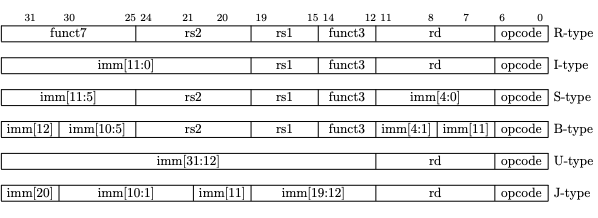
\includegraphics[width = \textwidth]{FormatiIstruzione.png}
	\caption{Formati istruzione RISC-V\cite{ISA}}
	\label{Fig:Formati_istruzioni_RV32I}
	
\end{figure}



In tutti i formati i registri sorgente (\textit{rs1} e \textit{rs2}) e il registro destinazione (\textit{rd}) vengono mantenuti nelle stesse posizioni per velocizzare la codifica.
L'ISA presenta 4 categorie di istruzioni:
\begin{itemize}
	\item \textbf{Istruzioni computazionali}: Sono presenti 21 istruzioni computazionali e vengono codificate nel formato R se è un'operazione tra i registri o nel formato I se è un'operazione tra registro e costante. Le istruzioni di questo tipo includono istruzioni aritmetiche, logiche e di comparazione sia per valore senza segno che per i valori con segno.
	\item \textbf{Accesso alla memoria}Le istruzioni di accesso alla memoria permettono il trasferimento di dati dalla memoria e alla memoria. Sono presenti 8 istruzioni in totale, 5 di load codificate nel formato I e 3 di store codificate nel formato S.
	\item \textbf{Controllo del flusso}Le istruzioni di controllo permettono di alterare il normale flusso sequenziale del programma. Sono presenti 6 istruzioni di questo tipo che permettono il trasferimento codificate nel formato B. Le istruzioni prevedono il confronto degli operandi in \textit{rs1} e \textit{rs2} e se la condizione è verificata viene aggiunto il valore del campo imm al \textit{program counter} per raggiungere l'indirizzo di arrivo.
	\item \textbf{Istruzioni di sistema}Con RV32I sono presenti 8 istruzioni di controllo del sistema. Possiamo dividerle in due gruppi. Il primo gruppo (ECALL, EBREAK) gestisce le \textit{system call}. Il secondo gruppo è utilizzato per leggere e scrivere i registri di stato.
\end{itemize}


\section{RV32I}
L'ISA base è stata progettata per supportare i moderni sistemi operativi. Questa base contiene 47 istruzioni uniche. I 32 registri sono di 32 bit (XLEN = 32) vengono identificati da x seguito da un numero. Il primo registro x0 contiene la costante zero e ogni istruzione che cerca di modificarlo solleva un eccezione. Gli altri registri x1 - x31 sono \textit{general purpose}. L'ABI definisce le convenzioni di utilizzo dei registri(Figura \ref{Fig:ConvenzioneRegistri}).

\begin{figure}[h!]
\centering
	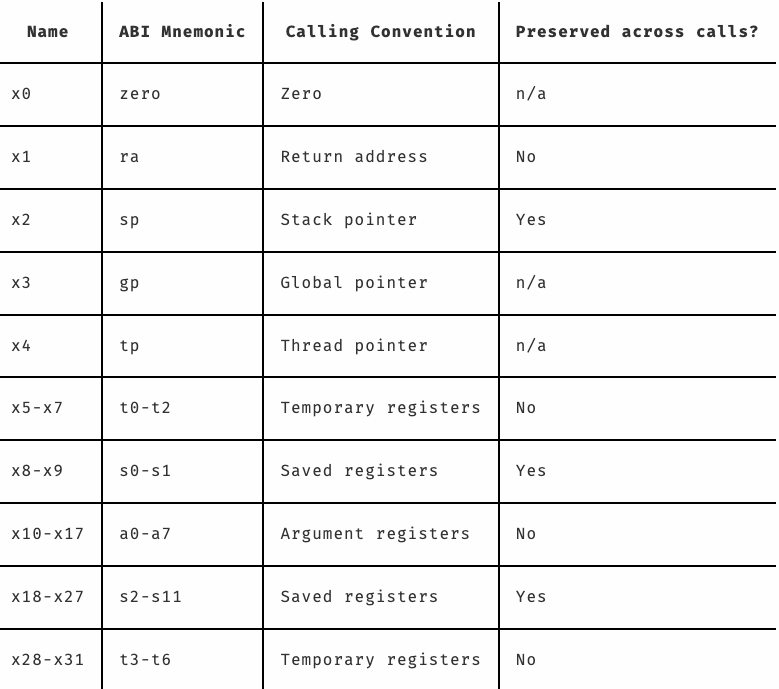
\includegraphics[scale=0.3]{ABI-RISC-V}
	\caption{Convenzione dei registri}
	\label{Fig:ConvenzioneRegistri}
\end{figure}

Come mostrato in Figura \ref{Fig:ConvenzioneRegistri} notiamo che non è presente un registro dedicato allo \textit{stack pointer} ne un \textit{return adress} ma vengono utilizzati rispettivamente il registro x2 e il registro x1.


\section{Le altre basi}
Esistono altri set che aumentano i bit utilizzati dai registri come RV64I e RV128I. 

%Sul documento che propone RISC-V sul proprio ISA vengono anche impostate le linee guida per fare delle proprie estensioni.



%%
%Capitolo 3: Compilatori
% cos è -> Storia -> Riguardo RISC-V -> due parole su gcc e clang

\chapter{Compilatori}
%\todo{atrent: riletto, sempre ignorando i numerosi errori ortgrafici e fraseologici}
\todo{Rileggere}
\section{Descrizione}
Un compilatore è un programma che trasforma il codice sorgente in linguaggio macchina. Il processo di compilazione prevede diverse fasi. La prima fase prevede un'analisi lessicale da cui vengono generati dei token. La seconda, utilizzando i token, prevede un'analisi sintattica e infine un'analisi semantica dopo la quale viene generato il codice intermedio. Questo codice intermedio attraversa una fase di ottimizzazione e infine viene generato il codice target \cite{GCC} \cite{LLVM}.


\begin{figure}
\centering
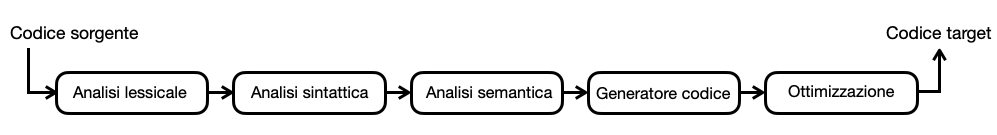
\includegraphics[width = \textwidth]{SchemaCompilatore.png}
\caption{Schema meccanismo di compilazione}
\label{Fig:MeccanismoCompilazione}
\end{figure}%\todo{fonte?} Questa l'ho fatta io 

Qualsiasi programma scritto in un linguaggio di programmazione di alto livello deve essere tradotto in codice oggetto prima di poter essere eseguito. Tutti i programmatori che utilizzano tale linguaggio utilizzano un compilatore o un interprete. I miglioramenti a un compilatore possono portare a un gran numero di funzionalità migliorate nei programmi eseguibili.

\section{Storia}
Il primo compilatore teorico fu pensato da Corrado Böhm che nel 1951 che lo sviluppò per la sua tesi di dottorato. Una prima implementazione di un compilatore è dovuta a Grace Hopper che ha anche coniato il termine ``compilatore''. Il programma, chiamato \textit{A-0 System}\cite{SystemA0}, funzionava come caricatore o linker, non come i moderni compilatori. \'E importante menzionare che il codice sorgente della versione A-2, datata 1953, fu rilasciato ai clienti con lo scopo di sviluppare dei miglioramenti. Possiamo dire che A-2 potrebbe essere considerato un esempio precoce di licenza libera \cite{openSource1, openOrg, stallman2003software}. 
%della filosofia del software libero e open source \cite{openSource1, openOrg, stallman2003software}. 

%\todo{aveva una licenza considerabile libera?!?} -> non ho trovato nessun riferimento al tipo di licenza.

\section{Cross-compilazione}
\label{Sec:Cross}
La cross-compilazione è il processo di compilazione del codice sorgente su un sistema diverso da quello in cui il codice verrà eseguito. In altre parole, il compilatore viene eseguito su una piattaforma diversa rispetto a quella di destinazione del software compilato. La cross-compilazione è spesso utilizzata nel contesto dello sviluppo di software per dispositivi embedded dove lo sviluppatore scrive il codice sorgente su un computer host più potente e poi lo compila per l'hardware a cui è destinato.


\section{Compilatori moderni}
Nell'ecosistema dei compilatori moderni i due pi\'u famosi sono: GCC e CLANG.
Il primo GCC (GNU Compiler Collection) fu creato nel 1987 ed oggi viene sviluppato da programmatori di tutto il mondo. Inizialmente nato per il linguaggio C oggi supporta altri linguaggi come Java, C++, Objective C \cite{GCCstory}.

Il secondo \'e nato nel 2005 e sviluppato da Apple Inc. Con lo scopo di avere un compilatore Apple ottimizzato per i loro dispositivi\cite{ClangStory}.

\section{Un buon compilatore} %
La scelta di un compilatore per un progetto è una scelta importante.I processori, oggi, sono strutturati in pipeline superscalari e in altre complesse strutture interne. Inoltre i linguaggi moderni astraggono dalla struttura hardware per ottenere un linguaggio logico più generale. Quindi si predilige un approccio meno specifico e non incentrato sulla struttura della macchina.Gli standard dei linguaggi, si fanno sempre più espressivi e astratti. Questa espressività dei linguaggi aumenta l'onere dei compilatori che devono essere in grado di generare un buon codice assembly. La selezione di un compilatore è una scelta cruciale per il proprio progetto. Si deve tener conto che la stessa porzione di codice, utilizzando compilatori differenti, può generare comandi assembly più o meno efficienti.
Oltre a generare programmi eseguibili ad alte prestazioni, i compilatori devono anche avere prestazioni elevate. Un progetto software di grandi dimensioni può contenere da centinaia a migliaia di singole unità di traduzione. Le unità di traduzione sono parti del codice sorgente che vengono tradotte dal compilatore in un file oggetto o in un file eseguibile. Ogni unità di traduzione può contenere migliaia di righe di codice. Oltre all'efficienza delle prestazioni del codice generato si deve tener conto anche del tempo in cui si genera il codice.

Quindi, un buon compilatore ci permette di concentrarci sul processo di programmazione piuttosto che farci preoccupare della struttura del sistema e deve essere in grado di produrre un codice che abbia delle buone performance in tempo relativamente breve.


\section{Toolchain di RISC-V}
In sistemi privi di un compilatore viene utilizzata la tecnica della \textbf{cross-compilazione}(Sezione \ref{Sec:Cross}). RISC-V mette a disposizione alcune \textit{toolchain} di compilazione. Una \textit{toolchain} è un insieme di programmi utilizzati sequenzialmente per la creazione di un software. In generale i programmi presenti sono un compilatore, un linker, un assembler, un debugger, un profiler, degli strumenti di analisi del codice e strumenti di gestione del progetto. Per RISC-V sono disponibili le \textit{toolchain gcc}\cite{toolchain_gcc} e \textit{toolchain clang}\cite{toolchain_clang}. Entrambe le \textit{toolchain} sono mantenute dalle community.Quella pi\'u aggiornata e utilizzata è quella del progetto GNU. Sul \href{https://wiki.riscv.org/display/HOME/RISC-V+Software+Ecosystem}{sito} sono elencate tutte le \textit{toolchain} disponibili e il sito offre una panoramica su tutto l'ecosistema RISC-V.


\subsubsection{GCC toolchain}
La toolchain GCC di RISC-V supporta linguaggi come C, C++, Objective-C, e Go. La versione corrente è la 12.2 (datata Agosto 2022). La toolchain ha aggionamenti molto di frequente. Ci sono quattro manutentori Andrew Waterman, Jim Wilson, Kito Cheng, Palmer Dabbelt .

\subsubsection{CLANG toolchain}
La toolchain LLVM/CLANG è sviluppata da \textit{lowRISC project} attualmente è alla versione 15.0.2. A differenza della \textit{toolchain gcc} è mantenuta solamente da Alex Bradbury.


%%%--------------------

\chapter{BenchMarking}
\todo{Rileggere}

Quando si parla di benchmark si intendono dei test di prova con lo scopo di fornire una valutazione delle prestazioni di un computer. In generale esistono due principali categorie di benchmark: sintetici o applicativi. I primi hanno lo scopo di misurare le prestazioni del sistema riguardo specifiche operazioni mentre gli ultimi si riferiscono a software applicativi. Come affermato da Wei Dai e Daniel Berleant in \textit{Benchmarking Contemporary Deep Learning Hardware and Frameworks: a Survey of Qualitative Metrics }\cite{benchmarkIntro} ci sono sette caratteristiche fondamentali che un benchmark deve avere:
\begin{enumerate}
 \item Rilevanza: i benchmark dovrebbero misurare caratteristiche importanti.
 \item Rappresentatività: le metriche delle prestazioni dovrebbero essere accettate dall'industria e dal mondo accademico.
 \item Equità: tutti i sistemi dovrebbero essere paragonati in modo equo.
 \item Ripetibilità: è possibile verificare i risultati dei benchmark.
 \item Rapporto costo-efficacia: i test di benchmark sono economici.
 \item Scalabilità: i test di benchmark dovrebbero funzionare sia su sistemi che possiedono poche risorse che numerose risorse.
 \item Trasparenza: le metriche utilizzate dovrebbero essere facili da capire.
\end{enumerate}
In questa sezione viene prima presentata la storia dei programmi di benchmark dalle origini fino a oggi presentando alcuni standard attuali dei benchmark. Successivamente vengono approfonditi alcuni benchmark utilizzati.

% Tipi di benchmark ... aggiungere ?
 
\section{Storia}
Il primo benchmark citato in letteratura prende il nome di Whetstone. I suoi autori, H.J. Curnow e B.A. Wichmann, svilupparono un programma con lo scopo di valutare le prestazioni in virgola mobile. Pubblicato nel 1976 questo benchmark fu il primo esempio di benchmark sintetico. La sua semplicità è data dalla sua organizzazione in moduli, ognuno specializzato per un aspetto.
 Un altro benchmark è LINPACK che risale al 1979(non pensato per\'o diventare un benchmark ). Questo benchmark utilizza una libreria \textit{BLAS (Basic Linear Algebra Subprograms) } per eseguire operazioni su vettori e su matrici per risolvere sistemi lineari. Lo scopo originale era quello di valutare le prestazioni in virgola mobile dei supercomputer dell'epoca ma poi fu utilizzato anche su architetture meno potenti\cite{LinpackSite}.
 Un altro benchmark simile è il famoso Dhrystone. Questo benchmark sintetico pubblicato nel 1984 ha lo scopo di valutare le prestazioni dei microprocessori e dei sistemi di elaborazione dati \cite{DhrystoneWP}.
 Tutti i programmi sviluppati prima dell'introduzione di Dhrystone erano pensati e scritti per valutare un unico aspetto. Il primo tentativo di avere un programma che valutasse pi\'u aspetti ci fu nel 1986. Il benchmark si chiama Livermore loops. Questo benchmark è composto da ventiquattro loop interni che valutano aspetti differenti. 
 Dopo lo sviluppo di un programma \textit{general purpose} si iniziò a pensare a delle suite di test che permettessero l'esecuzione solo di alcuni test per valutare determinati aspetti invece di un unico programma che svolgesse ogni valutazione pensata in fase di sviluppo.
Una delle prime raccolte di test degna di nota è la raccolta prodotta da \textit{Stanford University} e \textit{the University of California} quando in corrispondenza con la progettazione del primo sistema RISC furono raccolti piccoli programmi. Tra questi erano presenti programmi di: permutazione,  risoluzione di problemi come la torre di Hanoi, le otto regine,  puzzle e altri tipo moltiplicazione di matrici, quicksort, bubblesort, treesort, moltiplicazione di matrici con valori in virgola mobile e FFT (\textit{Fast Fourier Transform}).  L'importanza di questo \textit{Stanford Small Programs Benchmark Set} è dovuta al primo confronto tra architetture RISC e CISC \cite{CommonBench}.
%%
 Nel 1988 fu fondata una cooperativa con lo scopo di produrre benchmark validi lo SPEC \cite{SPECSite}.% imparziali, significativi e pertinenti. 
 I programmi utilizzati fino ad ora erano di piccole dimensioni e, con il miglioramento delle tecnologie, non potevano valutare le nuove architetture. Cos\'i fu fondato lo SPEC (\textit{The Standard Performance Evaluation Corporation}) il cui scopo era ed è quello di mantenere delle suite di test standardizzate per le nuove generazioni di computer. 
 Come nei sistemi comuni sono state sviluppate delle suite di test, cosi anche nel mondo riguarda il mondo embedded. Nel 1997 fu fondata EEMBC (\textit{l'Embedded Microprocessor Benchmark Consortium}) che, negli anni 2000, pubblicò una prima suite di test dedicati al mondo embedded \cite{EEMBCSite}. % nomi dei set in v1 ?
 Uno dei suoi prodotti più famosi \'e il benchmark chiamato CoreMark pubblicato nel 2009. %sezione core Mark
 Sempre nel mondo embedded fu creata la suite di test Embench, nel 2019 \cite{embenchSite}. Questa suite di test è stata sviluppata da altri progetti come \textit{The Bristol Embecosm Embedded Benchmark Suite (BEEBS)}, \textit{MiBench, the WCET benchmark collection, DSPstone, the Simple Generic Library} e\textit{the Nettle low-level cryptographic library}\cite{NettleSite}\cite{vittekBorovanskyMoreauTurin2006, }\cite{DSPStoneSite} \cite{WCETSite} \cite{MiBenchSite}. % BEEBES -> For the reasoning behind the choice of benchmarks in BEEBS, see BEEBS: Open Benchmarks for Energy Measurements on Embedded Platforms (https://arxiv.org/abs/1308.5174)
 
 %Quali sono gli standard di settore?
 Oggi gli tra gli standard di settore c'è il precedentemente citato SPEC, in particolare SPECint e SPECfp, il primo incentrato su prestazioni di calcolo con numeri interi e il secondo in virgola mobile. 
 Per quanto riguarda il mondo embedded, EEMBC è uno standard riconosciuto che, oltre a CoreMark, ha sviluppato altri benchmark mirati per dispositivi specifici (AutoBench per dispositivi automotive e industriali, Netwoking2.0 per router e switch e altri). % \cite{EEMBCSite}
 Altri standard di settore sono TPC (\textit{Transaction Processing Performance Council}) che si occupa di creare dei benchmark per i DBMS\cite{TPCSite}. %Meh

%Openbenchmark
 Oltre agli standard di settore, con gli anni, si sono sviluppati dei benchmark e delle suite di test open source. Un esempio \textit{phoronix test suite} \cite{ PhoronixTestSuiteSite}
 che supporta Linux, Windows Osx, e altri sistemi. Questa suite di test d\'a la possibilità di eseguire dei benchmark in maniera semplice(con l'unica richiesta di avere php da linea di comando ) e i risultati possono essere caricati su OpenBenchmark \cite{OpenBenchmarkSite}.



\section{Benchmark standard}


\subsection{CoreMark}
Per citare il sito ufficiale: 

\textit{CoreMark is a simple, yet sophisticated benchmark that is designed specifically to test the functionality of a processor core. Running CoreMark produces a single-number score allowing users to make quick comparisons between processors}. 

CoreMark è un benchmark che misura le prestazioni dei microcontrollori e delle CPU utilizzate nei sistemi embedded. In CoreMark sono implementati algoritmi di list processing, manipolazione di matrici, macchina a stati e CRC (controllo di ridondanza ciclico) . È progettato per funzionare su dispositivi da 8 bit a 64 bit\cite{CoreMark}.

CoreMark è un benchmark sintetico come Dhrystone e, come Dhrystone, CoreMark è piccolo, portatile, gratuito \footnote{La licenza di CoreMark è la "CoreMark License Agreement". La CoreMark License Agreement stabilisce che l'utente può utilizzare il benchmark CoreMark solo per scopi di valutazione delle prestazioni dei microprocessori e non per fini commerciali.} ma, a differenza di Dhrystone, CoreMark ha regole di esecuzione e reporting specifiche ed è stato progettato per evitare aspetti problematici di Dhrystone. Mentre Dhrystone risulta un benchmark del compilatore, CoreMark si focalizza sulle capacit\'a di lavoro della MCU o di una CPU \cite{analysis_EEMBC}.
Il codice sorgente è disponibile nel repository Github \footnote{\url{https://github.com/eembc/coremark} \cite{RepoCoreMark}}.
		

\subsection{LINPACK}
Il LINPACK Benchmark è una misura della velocità di esecuzione in virgola mobile di un computer. Viene determinato eseguendo un programma che risolve un denso sistema di equazioni lineari. Durante gli anni si sono sviluppate tre versioni di questo programma. 

La prima versione viene chiamata LINPACK 100 ed è molto simile alla versione del 1979. La soluzione si ottiene attraverso $ \frac{2}{3n^3} + 2n^2 $ operazioni in virgola mobile con n = 100. La seconda versione si chiama LINPACK 1000 e differentemente risolve problemi con n = 1000. L'ultima verisione chiamata HPL (\textit{High-Performance Linpack}) è dedicata ad una implementazione parallela di LINPACK\cite{LINPACK_PastPresFut} \cite{hplNetLib}.

% approfondisci	?

\section{Altri programmi} 

In questa sezione vengono presentati due programmi scritti da me che non sono standard di benchmarking. Il primo programma viene utilizzato per poi analizzare il codice assembly generato dal compilatore, mentre con il secondo vengono utilizzati degli algoritmi di sorting e comparato il tempo di esecuzione con gli stessi algoritmi eseguiti sul Raspberry.

%\todo{devi dichiarare l'autore e la motivazione}

\subsection{MultOrShift}
	Il programma confronta la velocità di esecuzione di moltiplicazione e divisione
aritmetiche con lo shift logico. Il programma genera un array di interi di
valori tra zero e maxInt e un array di potenze di due comprese tra due e
milleventiquattro. Entrambi gli array hanno mille elementi. Dopo la generazione
viene calcolato il risultato elemento per elemento e viene memorizzato il
tempo di esecuzione. Il risultato del programma \`e il tempo medio di esecuzione
di mille operazioni per tipo (moltiplicazione, divisione, 
moltiplicazione tramite shift, divisione tramite shift). 
Lo scopo di questo programma è osservare la differenza delle implementazioni delle operazioni a livello assembly compilato con la \textit{tool-chain} di RISC-V e confrontarle con le stesse operazioni compilate per ARM.
		
		
\subsection{Sorting}
Vengono utilizzati degli algoritmi di \textit{sorting} per confrontare il tempo di esecuzione sulla board con gli stessi algoritmi su Raspberry.Gli algoritmi di sorting utilizzati sono:
\begin{itemize}
	\item BubbleSort
	\item InsertionSort
	\item QuickSort
	\item HeapSort
\end{itemize}

Ogni algoritmo viene eseguito su array di dimensioni diverse: 500, 1000, 5000, 10000, 20000, 35000, 50000. Per ogni dimensione vengono eseguite 150 prove sulle quali viene calcolato il tempo di esecuzione. Il programma informa per ogni gruppo di array il tempo massimo, il minimo e il tempo medio. Per alcuni algoritmi vengono utilizzate anche delle configurazioni particolari dell'array da ordinare, come ad esempio utilizzando il BubbleSort vengono ordinati array strettamente crescenti e strettamente decrescenti oltre che ai campioni casuali. Nella situazione generale gli array vengono generati con numeri interi casuali.


\chapter{Comparativa}
\todo{Rileggere}

\section*{MacBook Air}
\label{sec:MacBook}
Per alcuni benchmark è stato utilizzato un MacBook Air per confronto. Il PC ha un processore 2, 2 GHz Intel Core i7 dual-core con memoria 8 GB 1600 MHz. Nelle sezioni successive i termini Pc fanno riferimento a questa architettura.

\section*{Raspberry Pi}

Il Raspberry Pi utilizzato è Raspberry Pi model B. La board datata 2013 è stata sviluppata come board scolastica e successivamente applicata a molti contesti come nel mondo embedded.
Con la dimensione di una carta di credito il Raspberry ha una RAM di 512 MB e una CPU da 700 MHz, due porte USB (Universal Serial Bus) e un'Ethernet. In aggiunta a ciò, ci sono pin di input/output (GPIO) per uso generico per collegare alcuni hardware. La tabella \ref{Tab:RaspSorting} mostra i tempi di esecuzione degli algoritmi di ordinamento eseguiti su Raspberry \cite{Rasp}.

\begin{figure}[ht]
\centering
	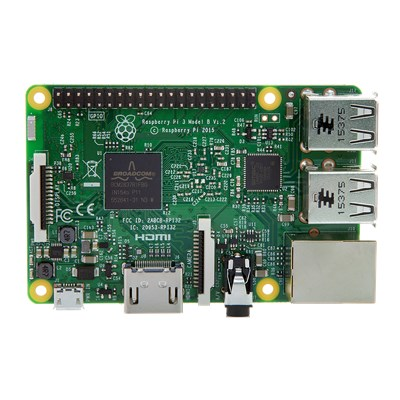
\includegraphics[scale=0.5 ]{RBTop.jpeg}
	\caption{Vista superiore Raspberry model B}
	\label{fig:RaspberryB}
\end{figure}

\section{CoreMark}
CoreMark è stato compilato con:

\begin{lstlisting}[language=sh, caption = {compilazione CoreMark}, captionpos = b]
./riscv64-unknown-elf-gcc -O2 -o coremark.exe core_list_join.c core_main.c core_matrix.c core_state.c core_util.c simple/core_portme.c -DPERFORMANCE_RUN=1 -DITERATIONS=1000
\end{lstlisting}



I codici sorgente sono stati compilati utilizzando alcuni file di configurazione per RISC-V presenti nella \href{https://github.com/riscv-boom/riscv-coremark}{repository}\cite{CoreMarkWrapper}. I file utilizzati non alterano la validità dell esecuzione di CoreMark
\cite{CoreMarkRepo}.

Il programma è stato eseguito quindici volte con i seguenti risultati:


\begin{table}[ht]
\begin{tabular}{|l|l|l|l|l|l|l|l|}
\hline
  & Score       &   & Score       &    & Score       &    & Score       \\ \hline
1 & 2312,479985 & 5 & 2311,881624 & 9 & 2311,874448 & 13 & 2311,444275 \\ \hline
2 & 2312,596169 & 6 & 2311,149103 & 10 & 2311,432578 & 14 & 2310,397101 \\ \hline
3 & 2311,137567 & 7 & 2310,215865 & 11 & 2311,265017 & 15 & 2311,553826 \\ \hline
4 & 2311,144929 & 8 & 2312,048460 & 12 & 2311,013694 &  &  \\ \hline
\end{tabular}
\caption{Score di CoreMark ad ogni esecuzione}
\end{table}


\begin{table}[ht]
\centering
\begin{tabular}{|l|c|}
\hline
Media & 2311, 307997 \\ \hline
Dev.std & 0, 754112 \\ \hline
\end{tabular}
\caption{Score medio e deviazione standard di CoreMark}
\end{table}


\begin{table}
\centering
\begin{tabular}{|l|l|l|l|l|l|l|}
\hline
&
 Cortex A72 &
 BCM2837 &
 BCM2835 &
 D1 &
 A20 &
 X1000E 
 \\ \hline
CoreMark & 48.626 & 15.364 & 1.303, 8 & 2.240, 8 & 2.086, 2 & 2.231, 1 \\ \hline
CoreMark/MHz & 22, 670 & 12, 803 & 1, 8625 & 2, 2408 & 2, 0862 & 2, 2311 \\ \hline
\end{tabular}
\end{table}

\section{LINPACK}
Il benchmark sia nella versione LINPACK100 che LINPACK1000 è stato compilato con:

\begin{lstlisting}[language=sh, caption = {compilazione LINPACK}, captionpos = b]
gcc -O4 -DDP -DROLL -o linpackc linpack.c -lm
\end{lstlisting}


Il programma è stato eseguito quindici volte con i seguenti risultati:

\begin{table}[ht]
\begin{tabular}{|l|l|l|l|l|l|l|l|}
\hline
  & MFLOPS     &   & MFLOPS     &    & MFLOPS     &    & MFLOPS     \\ \hline
1 & 169,004840 & 5 & 163,725958 & 9 & 170,431042 & 13 & 175,125393 \\ \hline
2 & 166,062072 & 6 & 161,682756 & 10 & 175,125393 & 14 & 175,528289 \\ \hline
3 & 168,424495 & 7 & 163,999682 & 11 & 173,313142 & 15 & 173,094698 \\ \hline
4 & 168,672726 & 8 & 169,840877 & 12 & 175,573170 &  &  \\ \hline
\end{tabular}
\end{table}

\begin{table}[ht]
\centering
\begin{tabular}{|l|l|l|}
\hline
N & 100 & 1000 \\ \hline
Media & 170, 098131 & 120, 066523 \\ \hline
Dev.std & 4, 565740 & 0, 282790 \\ \hline
\end{tabular}
\caption{MFLOPS LINPACK}
\end{table}

\begin{table}[ht]
\centering
\begin{tabular}{|l|l|l|}
\hline
N & 100 & 1000 \\ \hline
Media & 0, 004040 & 5, 569164 \\ \hline
Dev.std & 0, 000109 & 0, 013134 \\ \hline
\end{tabular}
\caption{Tempo di risoluzione LINPACK}
\end{table}

\section{MultOrShift}
Il programma confronta la velocità di esecuzione di moltiplicazione e divisione aritmetiche con lo shift. Il programma genera un array di interi di valori tra zero e maxInt e un array di potenze di due comprese tra due e milleventiquattro. Entrambi gli array hanno mille elementi. Dopo la generazione viene calcolato elemento per elemento il risultato e viene memorizzato il tempo di esecuzione. Il risultato del programma è il tempo medio di esecuzione di mille operazioni per tipo (moltiplicazione normale, divisione normale, moltiplicazione tramite shift, divisione tramite shift). Di seguito alcune porzioni di codice:

\lstinputlisting[language=c, style = Cstyle, caption = Impostazioni dei dati, label ={Code:Init} ]{PorzioniCodice/MultShift/init.c}
\lstinputlisting[language=c, style = Cstyle, caption = Moltiplicazione, label ={Code:Mult} ]{PorzioniCodice/MultShift/Mult.c}
\lstinputlisting[language=c, style = Cstyle, caption = Shift, label ={Code:Shift} ]{PorzioniCodice/MultShift/Shift.c}

Il codice \ref{Code:Init} imposta i due array. I codici \ref{Code:Mult} e \ref{Code:Shift} mostrano l'operazione eseguita.
La tabella \ref{Tab:tempi_esecuzioneMS} mostra i tempi di esecuzione calcolati in millisecondi delle varie operazioni.

\begin{table}[ht]
\centering
\begin{tabular}{lcccc}
\cline{2-5}
\multicolumn{1}{l|}{} & \multicolumn{2}{c|}{PC} & \multicolumn{2}{c|}{RISC-V} \\ \hline
\multicolumn{1}{|l|}{Normale} & \multicolumn{1}{c|}{0.0036} & \multicolumn{1}{c|}{0.0042} & \multicolumn{1}{c|}{0.0430} & \multicolumn{1}{c|}{0.0572} \\ \hline
\multicolumn{1}{|l|}{Shift} & \multicolumn{1}{c|}{0.0034} & \multicolumn{1}{c|}{0.0034} & \multicolumn{1}{c|}{0.0404} & \multicolumn{1}{c|}{0.0826} \\ \hline
 & \multicolumn{1}{l}{} & \multicolumn{1}{l}{} & \multicolumn{1}{l}{} & \multicolumn{1}{l}{} 
\end{tabular}
	\caption{Tempi di esecuzione operazioni calcolati in ms}
	\label{Tab:tempi_esecuzioneMS}
\end{table}
	
	
\section{Analisi codice assembly}
Per capire meglio i risultati osserviamo e compariamo i codici generati dai compilatori. I Compilatori confrontati sono \textit{gcc RISC-V}, \textit{gcc ARM} e \textit{gcc x86\_64}. I compilatori RISC-V e ARM vengono confrontati per il loro focus sul'ambiente embedded ed entrambi sono architetture RISC.Tutti i codici presentati in questa sezione vengono compilati e presentati con il livello di ottimizzazione di default (-O0) \cite{ConfrontoISABook}.


\subsection{Addizione con costante}

\lstinputlisting[language=c, style = Cstyle, caption = Addizione, label = {Code:AddComp}]{PorzioniCodice/ConfrontoCompilatori/C/get_num.c}

La funzione è una semplice funzione scritta in C che dato un numero di tipo intero restituisce il numero sommato a ventitré \footnote{La scelta del numero è puramente casuale}.
  
\vspace{0.3 cm}
\textbf{RISC-V}

\vspace{0.3 cm}
Il sorgente compilato con il compilatore RISC-V \ref{Code:AddRISCV} da riga due fino a riga sei, predispone la chiamata della procedura posizionando sullo stack il necessario. Da riga sette inizia la funzione. Su quella riga viene recuperato il valore di \textit{num} che alla riga otto, tramite l'operazione di add immediate, viene sommato a num. Il risultato dell'operazione addiw è la somma del valore di num sommato alla costante ventitré. Il risultato è esteso su sessantaquattro bit e vengono ignorati gli errori di overflow. Successivamente tramite la pseudo-istruzione sext.w prende i 32 bit inferiori e li memorizza nel registro rd. Questa istruzione corrisponde a addiw rd, rs, 1 0. Il risultato viene spostato nel registro a0 che, nei processori RISC-V, viene utilizzato come restituzione di risultato. Le righe successive ripristinano lo stack e restituiscono il controllo al chiamante.

\vspace{0.3 cm}
\textbf{ARM}

\vspace{0.3 cm}

Il sorgente \ref{Code:Addx86}, compilato con gcc ARM, mostra che la preparazione della procedura si esegue da riga due a riga cinque.Con le due righe successive si esegue la funzione. La riga sei recupera il valore di num. La riga successiva calcola il valore del risultato e, infine, alla riga otto si sposta il risultato nel registro di restituzione


\vspace{0.3 cm}
\textbf{x86}

Il sorgente \ref{Code:AddARM} è compilato con gcc di x86. Da riga due fino a riga quattro viene preparato lo stack, a riga cinque viene posizionato num nel registro eax e a riga sei viene sommato a ventitré e memorizzato nel registro eax. Infine viene ridato il controllo al chiamante.

\vspace{0.3 cm}

\begin{figure}[ht]
 
 \begin{subfigure}{0.3\textwidth}
 
 \lstinputlisting[language = Risc-v, caption = {RISC-V}, label = {Code:AddRISCV} ]{PorzioniCodice/ConfrontoCompilatori/Assembler/RISC-V/get_num.txt}


 \end{subfigure}
 \hfill
 \begin{subfigure}{0.3\textwidth}
 
 \lstinputlisting[language = Risc-v, caption = {Arm}, label = {Code:AddARM}]{PorzioniCodice/ConfrontoCompilatori/Assembler/ARM/get_num.txt}


 \end{subfigure}
 \hfill
 \begin{subfigure}{0.3\textwidth}
 
 \lstinputlisting[language = Risc-v, caption = {x86}, 	label = {Code:Addx86}]{PorzioniCodice/ConfrontoCompilatori/Assembler/x86/get_num.txt}


 \end{subfigure}
 
 \caption{Funzione di somma}
 
\end{figure}

\subsection{Addizione}
Nel caso generale viene calcolata la somma di tre numeri.
\lstinputlisting[language=C, style = Cstyle, caption = {Addizione generale}, label = {Code:Add2Comp}]{PorzioniCodice/ConfrontoCompilatori/C/sumGen.c}


\vspace{0.3 cm}
\textbf{RISC-V}

Nel caso del compilatore RISC-V la somma avviene tra riga tredici e riga diciannove dove gli operandi vengono caricati nei registri a4 e a5 e successivamente calcolato il risultato e memorizzato in a4 che poi verrà sommato con l'ultimo operando, caricato a riga diciassette.

\vspace{0.3 cm}
\textbf{ARM}

Nel caso ARM avviene lo stesso meccanismo. Tra le righe otto e dodici avviene il caricamento dei primi due operandi e la somma parziale e infine la somma totale.

\vspace{0.3 cm}
\textbf{x86}

Infine per x86 il calcolo avviene tra le righe sette e undici nello stesso modo con cui viene eseguito in ARM.

\begin{figure}[ht]
 
 \begin{subfigure}[b]{0.3\textwidth}
 
 \lstinputlisting[language = Risc-v, caption = RISC-V] {PorzioniCodice/ConfrontoCompilatori/Assembler/RISC-V/sumGen.txt}
	\label{Code:Add2RISC}
\caption{RISC-V}
 \end{subfigure}
 \hfill
 \begin{subfigure}[b]{0.3\textwidth}
 
 \lstinputlisting[language = Risc-v, caption = ARM]{PorzioniCodice/ConfrontoCompilatori/Assembler/ARM/sumGen.txt}
 \label{Code:Add2ARM}

 \end{subfigure}
 \hfill
 \begin{subfigure}[b]{0.3\textwidth}
 
 \lstinputlisting[language = Risc-v, caption = x86]{PorzioniCodice/ConfrontoCompilatori/Assembler/x86/sumGen.txt}
	 
	\label{Code:Add2X86}
 \end{subfigure}
 
 \caption{Funzione di somma}
 \label{Fig:code2}
\end{figure}



\subsection{Moltiplicazione}

\vspace{0.3 cm}
\textbf{Moltiplicazioni per potenze di 2}

\lstinputlisting[language=C, style = Cstyle, caption = {Moltiplicazione per potenza di 2}, label = {Code:Mul2Comp}]{PorzioniCodice/ConfrontoCompilatori/C/mult2.c}

La funzione "dato un numero di tipo intero" restituisce il numero moltiplicato per due. Per i sorgenti le parti di preparazione sono simili alle rispettive preparazioni precedenti.


\vspace{0.3 cm}
Nei sorgenti in figura \ref{Fig:code2} viene mostrata l'operazione di moltiplicazione per due. Questa avviene per RISC-V e per ARM tramite uno shift logical left di un bit (SLLIW) mentre per x86 avviene tramite una somma. Questa somma è un caso particolare: infatti se volessimo moltiplicare per una qualsiasi potenza di due,  le operazioni avvengono tutte tramite shift left di un opportuno valore. Con la figura \ref{Fig:mult8} viene mostrato il calcolo di una moltiplicazione per otto. In tutti i casi il calcolo avviene attraverso Shift.


\vspace{0.3 cm}

\begin{figure}
 
 \begin{subfigure}[b]{0.3\textwidth}
 
 \lstinputlisting[language = risc-v, caption = RISC-V]{PorzioniCodice/ConfrontoCompilatori/Assembler/RISC-V/mult2.txt}
 

	\label{Code:Mul2RISC}
 \end{subfigure}
 \hfill
 \begin{subfigure}[b]{0.3\textwidth}
 
 \lstinputlisting[language = risc-v, caption = ARM]{PorzioniCodice/ConfrontoCompilatori/Assembler/ARM/mult2.txt}	
	
		\label{Code:Mul2ARM}
 \end{subfigure}
 \hfill
 \begin{subfigure}[b]{0.3\textwidth}
 
 \lstinputlisting[language = risc-v, caption = x86]{PorzioniCodice/ConfrontoCompilatori/Assembler/x86/mult2.txt}

	\label{Code:Mul2X86}
 \end{subfigure}
 \caption{Moltiplicazione per 2}
 \end{figure}
 	
 \begin{figure}
 \begin{subfigure}[b]{0.3\textwidth}
 
 \lstinputlisting[language = risc-v, caption = RISC-V]{PorzioniCodice/ConfrontoCompilatori/Assembler/RISC-V/mult8.txt}	
		
		\label{Code:Mul8RISC}
 \end{subfigure}
 \hfill
 \begin{subfigure}[b]{0.3\textwidth}
 
 \lstinputlisting[language = risc-v, caption = ARM]{PorzioniCodice/ConfrontoCompilatori/Assembler/ARM/mult8.txt}	

		\label{Code:Mul8ARM}
 \end{subfigure}
 \hfill
 \begin{subfigure}[b]{0.3\textwidth}
 
 \lstinputlisting[language = risc-v, caption = x86]{PorzioniCodice/ConfrontoCompilatori/Assembler/x86/mult8.txt}	

		\label{Code:Mul8X86}
 \end{subfigure}
 
 \caption{Moltiplicazione per 8}
 \label{Fig:mult8}
\end{figure}

\vspace{0.3 cm}

\textbf{Moltiplicazione per una costante}

Vengono presentati due codici: il primo moltiplica per un numero che dista da una potenza di due solamente uno, il secondo che dista di due. I numeri presi per questo esempio sono trentuno, nel primo caso, e trenta nel secondo.

\vspace{0.2 cm }

\begin{figure}[ht]
	\begin{subfigure}[b]{0.4\textwidth}
 
 \lstinputlisting[language=C, style = Cstyle, label = {Code:Mul31Comp}, caption = {moltiplicazione per 31}]{PorzioniCodice/ConfrontoCompilatori/C/mult31.c}	
		
 \end{subfigure}
 \hfill
 \begin{subfigure}[b]{0.4\textwidth}
 
 \lstinputlisting[language=C, style = Cstyle, label = {Code:Mul30Comp}, caption = {moltiplicazione per 30}]{PorzioniCodice/ConfrontoCompilatori/C/mult30.c}	
		
 \end{subfigure}
 
\end{figure}

\vspace{0.3 cm}
%%%%%
Nel caso della moltiplicazione per trentuno l'approccio dei tre sorgenti è identico. Viene calcolata la moltiplicazione per trentadue attraverso shift logici e poi viene sottratto una volta il valore per ottenere la moltiplicazione per trentuno. Se il valore costante fosse trentatré, il numero successivo alla potenza di due, l'operazione di sottrazione viene sostituita con una di addizione. Nel secondo caso abbiamo un approccio differente.

Partendo dal x86 la moltiplicazione avviene semplicemente con l'istruzione imul a riga sei. Nel caso ARM l'operazione di moltiplicazione viene comunque eseguita da una singola istruzione(riga otto) ma vengono utilizzati i registri r2 e r3 che precedentemente (riga sei e sette) vengono riempiti con gli operandi. Infine l'implementazione di RISC-V utilizza ancora shift. Nel caso della moltiplicazione per trenta avviene prima uno shift di quattro ( moltiplicazione per sedici) successivamente sottratto una volta il numero e infine al risultato avviene applicato uno shift di uno (moltiplicazione per due). Quindi: 
\begin{center}
	\vspace{0.2cm}
$((num * 2^4) - num ) * 2^1 = $ 

$ =((num * 16 ) - num ) * 2 =$ 

$ = 15 * num * 2 = num *30 $ 
\end{center}


\vspace{0.2 cm}
In generale RISC-V utilizza opportuni shift combinate con addizioni e sottrazioni per ottenere il valore della costante.

\begin{figure}[h]

 \begin{subfigure}[b]{0.3\textwidth}
 
 \lstinputlisting[language = risc-v, caption = {RISC-V}]{PorzioniCodice/ConfrontoCompilatori/Assembler/RISC-V/mult31.txt}
 \label{Code:Mul31RISC}


 \end{subfigure}
 \hfill
 \begin{subfigure}[b]{0.3\textwidth}
 
 \lstinputlisting[language = risc-v, caption = ARM]{PorzioniCodice/ConfrontoCompilatori/Assembler/ARM/mult31.txt}	
		
		 \label{Code:Mul31ARM}
 \end{subfigure}
 \hfill
 \begin{subfigure}[b]{0.3\textwidth}
 
 \lstinputlisting[language = risc-v, caption = x86]{PorzioniCodice/ConfrontoCompilatori/Assembler/x86/mult31.txt}
	
	 \label{Code:Mul31X86}
 \end{subfigure}
 \caption{Moltiplicazione per 31}
 \end{figure}

\begin{figure}

 \begin{subfigure}[b]{0.3\textwidth}
 
 \lstinputlisting[language = risc-v, caption = RISC-V]{PorzioniCodice/ConfrontoCompilatori/Assembler/RISC-V/mult30.txt}
 \label{Code:Mul30RISC}
	

 \end{subfigure}
 \hfill
 \begin{subfigure}[b]{0.3\textwidth}
 
 \lstinputlisting[language = risc-v, caption = ARM]{PorzioniCodice/ConfrontoCompilatori/Assembler/ARM/mult30.txt}	
		
		 \label{Code:Mul30ARM}
 \end{subfigure}
 \hfill
 \begin{subfigure}[b]{0.3\textwidth}
 
 \lstinputlisting[language = risc-v, caption = x86]{PorzioniCodice/ConfrontoCompilatori/Assembler/x86/mult30.txt}
	
	 \label{Code:Mul30X86}
 \end{subfigure}
 \caption{Moltiplicazione per 30}
 \end{figure}

\vspace{2cm}

\subsection{Divisione}
Per quanto riguarda la divisione viene utilizzato la stessa metodologia della moltiplicazione.

\subsection{Confronto ISA}
Le ISA, RISC-V e ARM, prese in esame hanno un approccio RISC. 

\todo{ISA femminile -\> controlla generi}
Molte ISA di tipo RISC utilizzano la stessa struttura di pipeline per le proprie implementazioni architetturali e non \'e da meno RISC-V. La struttura di questa ISA \'e caratterizzata da una pipeline a 5 \textit{stages}. In ogni fase della pipeline l'istruzione compie una determinata azione che permette l'esecuzione quasi parallela. %\todo{controlla che si dica cosi}
%confronto pipeline e non-pipeline
%...
Le cinque fasi della pipeline RISC-V sono \textit{Istruction fetch}, \textit{Istruction decode}, \textit{Execute}, \textit{Memory access}, \textit{Writeback}. %spiega le fasi
Naturalmente la parziale parallelizzazione del codice non evita situazioni critiche(\textit{Hazard}) che vengono risolte tramite le tecniche di \textit{Bypassing} e l'\textit{Interlock}. Queste situazioni critiche portano a modifiche necessarie a livello di struttura ma comportano un miglioramento di esecuzione del codice \footnote{Nel nostro caso in esame il core della CPU D1-H \'e XuanTie C906 \cite{DocH1}, ha una pipeline a 5 \textit{stages}}. 
%architetture ARM 
Per quanto riguarda ARM abbiamo avuto dei miglioramenti.  Inizialmente le pipeline ARM erano organizzate in pipeline a 3 \textit{stages}: \textit{Istruction fetch}, \textit{Istruction decode, Execute}. In questa situazione tre istruzioni diverse possono occupare ognuno dei tre stadi. L’hardware di ogni stadio deve poter operare in maniera indipendente. Con questa struttura quando il processore esegue istruzioni di \textit{data processing} la latenza massima \'e pari ai tre cicli e il throughtput \'e una sola istruzione, inoltre, ogni istruzione di trasferimento dati causa uno stallo della pipeline \cite{3stagesPipeline}. Avendo la memoria unica per dati e per le istruzioni non è possibile leggere l’istruzione successiva mentre si leggono dati.Quindi aumenta la latenza. Solamente dal ARM9TDMI\footnote{La nomenclatura del processore identifica le specifiche dello stesso. 9: Serie, T: Thumb ; D: Debugger; M: Moltiplicatore; I: ICE Macrocel integrato;} la pipeline è diventata a 5 stadi avendo le caratteristiche precedentemente citate.

%
%Immagine
Le architetture ARM con focus nel embedded sono caratterizzate da una pipeline a 3 stadi. 

%CPI
\begin{table}[ht]
\centering
\begin{tabular}{|l|l|l|l|}
\hline
RISC-V   & Clock & Linee & CPI  \\ \hline
get\_num & 17    & 12    & 1.41 \\ \hline
sumgen   & 24    & 22    & 1.09 \\ \hline
mult2    & 17    & 12    & 1.41 \\ \hline
mult8    & 17    & 12    & 1.41 \\ \hline
mult30   & 20    & 15    & 1.33 \\ \hline
mult31   & 20    & 14    & 1.42 \\ \hline
\end{tabular}
\caption{CPI per RISC-V}
\label{tab:CPI_RISCV}
\end{table}

\begin{table}[ht]
\centering
\begin{tabular}{|l|l|l|l|}
\hline
ARM  & Clock & Linee & CPI  \\ \hline
get\_num & 27    & 11    & 2.45 \\ \hline
sumgen   & 31    & 16    & 1.93 \\ \hline
mult2    & 21    & 11    & 1.9  \\ \hline
mult8    & 21    & 11    & 1.9  \\ \hline
mult30   & 25    & 12    & 2.08 \\ \hline
mult31   & 25    & 13    & 1.92 \\ \hline
\end{tabular}
\caption{CPI per ARM}
\label{tab:CPI_ARM}
\end{table}

\begin{table}[ht]
\centering
\begin{tabular}{|l|l|l|}
\hline
CPI  & RISC-V & ARM   \\ \hline
get\_num & 1.41 & 2.25     \\ \hline
sumgen   & 1.09 & 1.93     \\ \hline
mult2    & 1.41 & 1.9      \\ \hline
mult8    & 1.41 & 1.9      \\ \hline
mult30   & 1.33 & 2.08   \\ \hline
mult31   & 1.42 & 1.92  \\ \hline
\end{tabular}
\caption{CPI a confronto}
\label{tab:CPI_RISC-V_ARM}
\end{table}

\begin{table}[h]
\centering
\begin{tabular}{|l|l|l|l|l|l|l|}
\hline
Dimensione codice & get\_num & sumGen & mult2 & mult8 & mult30 & mult31 \\ \hline
ARM           & 2546     & 2896   & 2535  & 2537  & 2584   & 2569   \\ \hline
RISC-V               & 3295     & 3588   & 3284  & 3286  & 3306   & 3322   \\ \hline
\end{tabular}
\caption{Code size in byte [B]}
\end{table}

Le tabelle \ref{tab:CPI_RISCV} e \ref{tab:CPI_ARM} mostrano i clock richiesti per eseguire ogni programma. La tabella \ref{tab:CPI_RISC-V_ARM} confronta diretamente i CPI delle architetture. Dalle tabelle possiamo capire che pur avendo un numero di linee di codice maggiore e una dimensione maggiore, RISC-V riesce, grazie alla struttura in 5 stages, ad avere un numero di clock per esecuzione minore rispetto a ARM. %alcuni numeri




%\todo{atrent: manca una analisi, hai solo mostrato come vengono tradotte in assembly, ma non metti commenti}
%\todo{mattia: Qui non so come continuare atrent: basta che man mano che descrivi i confronti fra i due assembly dici qualche parola di commento, ad esempio sulla lunghezza del codice vs. cicli di clock per l'esecuzione vs. memoria occupata}
%\todo{mattia: questo è altro materiale online: \href{https://www.electropages.com/blog/2021/03/arm-vs-risc-v}{sit}
%atrent: mi sembra buono, puoi usare le parti interessanti citando in footnote il blogpost}
\todo{mattia: aggiunto alla fine qualche parola di commento(CPI, lunghezza, dimensione) }

\newpage
\section{Sorting}
Gli algoritmi di ordinamento sono una parte importante dell'elaborazione dei dati e sono ampiamente utilizzati in molti aspetti ad esempio in crittografia e nella ricerca di informazioni. Esistono molti tipi di algoritmi di ordinamento e ognuno ha i suoi vantaggi e limiti. In informatica, l'algoritmo di ordinamento è solitamente classificato per:

\begin{itemize}
	\item Complessità temporale. %Si basa su quanti valori si ha da distribuire. Questi vengono indicati con n.Possiamo avere una prestazione buona come $\mathcal{O}(n\log{}n)$ oppure peggiore come $\mathcal{O}(n!)$.
	\item Memoria utilizzata.
	\item Stabilit\'a.% ovvero se viene preservato l'ordine relativo dei dati con chiavi uguali all'interno dei valori da ordinare.
\end{itemize}

In base alle proprietà dei diversi tipi di dati, l'efficienza può essere migliorata scegliendo algoritmi di ordinamento appropriati. In questo capitolo verranno descritti quattro algoritmi di ordinamento e verranno analizzati comparandoli all'esecuzione su raspberry. L'ordinamento a cui si fa riferimento nelle sezioni successive è un ordinamento di array da mettere in ordine non decrescente.

\subsection{Bubble sort}
Bubble sort è un semplice algoritmo di ordinamento. 
L'algoritmo funziona nel modo seguente:
\begin{enumerate}
	\item Confronta gli elementi adiacenti, se il primo è maggiore del secondo, scambiali.
	\item Ripeti il primo punto dal secondo numero fino alla fine.
	\item Ripeti i primi due passaggi tante volte quanti elementi da riordinare.
\end{enumerate}

L'efficienza dell'algoritmo è basata sull'ordinamento dell'array da ordinare. Nel caso migliore l'array è gia ordinato e, passandolo all'algoritmo, esegue solo il punto 1 dall'inizio alla fine. Al contrario il caso peggiore è quando l'array si trova nell'ordine non crescente.
\begin{table}[ht]
	\centering
	\begin{tabular}{lc}
 & Complessità \\
Caso peggiore & $ \mathcal{O}(n^2)$ \\
Caso migliore & $ \mathcal{O}(n)$ \\
\end{tabular}
	\caption{complessit\'a bubble sort}
	\label{Tab:CompBubbleSort}
\end{table}

Di seguito viene riportato il codice (Code \ref{Code:BubbleSort}) dell'algoritmo e i tempi di esecuzione(Tab \ref{Tab:Tempi esecuzione Bubblesort}) secondo la dimensione dell'array e la situazione iniziale dell'array:
\lstinputlisting[language=C, style = Cstyle, caption = {Algoritmo bubble sort scritto in c}, label = {Code:BubbleSort}]{PorzioniCodice/Sorting/Bubble.c}	

\begin{table}[ht]
\centering
\begin{tabular}{| l | l | l | l |}
\hline
 & Caso peggiore & Caso migliore & Caso Generale \\ \hline
500 & 0.009426 & 0.004667 & 0.007156 \\ \hline
1000 & 0.037558 & 0.018877 & 0.028745 \\ \hline
5000 & 0.941429 & 0.470478 & 0.718178 \\ \hline
10000 & 3.784664 & 1.893387 & 2.889989 \\ \hline
20000 & 15.249109 & 7.639312 & 11.617705 \\ \hline
35000 & 46.744558 & 23.460390 & 35.640101 \\ \hline
50000 & 95.389578 & 47.888541 & 72.735791 \\ \hline
\end{tabular}
\caption{Tempi di esecuzione bubble sort in ms}
\label{Tab:Tempi esecuzione Bubblesort}
\end{table}

\newpage
\subsection{Insertion sort}
L'algoritmo consiste nel considerare un elemento alla volta, inserendolo nella posizione corretta tra gli elementi che sono gi\'a stati ordinati. 
\begin{table}[ht]
	\centering
	\begin{tabular}{lc}
 & Complessità \\
Caso peggiore & $ \mathcal{O}(n!)$ \\
Caso migliore & $ \mathcal{O}(n)$ \\
Caso medio & $ \mathcal{O}(n!)$\\
\end{tabular}
	\caption{complessit\'a insertion sort}
	\label{Tab:CompInsertionSort}
\end{table}


\lstinputlisting[language=C, style = Cstyle, caption = {Algoritmo bubble sort scritto in c}, label = {Code:InsertionSort}]{PorzioniCodice/Sorting/Insertion.c}	

Come nel caso del bubble sort è riportato anche il tempo di esecuzione nel caso peggiore e migliore.

\begin{table}[ht]
\centering
\begin{tabular}{| l | l | l | l |}
\hline
 & Caso peggiore & Caso migliore & Caso Generale \\ \hline
500 & 0.005423 & 0.000028 & 0.002634 \\ \hline
1000 & 0.020836	 & 0.000055 & 0.010575 \\ \hline
5000 & 0.521686 & 0.000287 & 0.260862 \\ \hline
10000 & 2.103697 & 0.000645 & 1.048553 \\ \hline
20000 & 8.497346 & 0.001114 & 4.220421 \\ \hline
35000 & 26.066370 & 0.001928 & 12.969309 \\ \hline
50000 & 53.187672 & 0.002720 & 26.499820 \\ \hline

\end{tabular}
\caption{Tempi di esecuzione insertion sort in ms}
\label{Tab:Tempi esecuzione InsertionSort}
\end{table}


\subsection{QuickSort}
L'algoritmo quicksort è un algoritmo ricorsivo del tipo divide et impera. L'algoritmo si basa:

\begin{enumerate}
\item Scegli un pivot dagli elementi dell'array.
\item Ordina l'array. Se l'elemento è più grande del pivot, allora mettilo dopo il pivot, altrimenti prima.
\item Ripetere questi due passaggi per i sottoarray finché ogni elemento non è nell'ordine corretto.
\end{enumerate}

Il tempo di esecuzione nel caso peggiore \'e $\mathcal{O}(n!) $, il tempo di esecuzione medio di quicksort è $\mathcal{O}(n * \log{}n) $. In seguito viene mostrata l'implementazione 

\lstinputlisting[language=C, style = Cstyle, caption = {Algoritmo quick sort scritto in c}, label = {Code:QuickSort}]{PorzioniCodice/Sorting/Quick.c}	

\begin{table}[ht]
\centering
\begin{tabular}{| l | l |}
\hline
 & Tempo \\ \hline
500 & 0.000273 \\ \hline
1000 & 0.000610 \\ \hline
5000 & 0.003813 \\ \hline
10000 & 0.008423 \\ \hline
20000 & 0.017266 \\ \hline
35000 & 0.032285 \\ \hline
50000 & 0.048096 \\ \hline

\end{tabular}
\caption{Tempi di esecuzione quick sort in ms}
\label{Tab:Tempi esecuzione QuickSort}
\end{table}

\subsection{Heap sort}
L'heapsort è un algoritmo di ordinamento iterativo, l'implementazione utilizzata è in-place.

\lstinputlisting[language=C, style = Cstyle, caption = {Algoritmo heap sort scritto in c}, label = {Code:HeapSort}]{PorzioniCodice/Sorting/Heap.c}	

\begin{table}[ht]
\centering
\begin{tabular}{| l | l |}
\hline
 & Tempo \\ \hline
500 & 0.000569 \\ \hline
1000 & 0.001272 \\ \hline
5000 & 0.008016 \\ \hline
10000 & 0.017815 \\ \hline
20000 & 0.041886 \\ \hline
35000 & 0.083366 \\ \hline
50000 & 0.128863 \\ \hline

\end{tabular}
\caption{Tempi di esecuzione heap sort in ms}
\label{Tab:Tempi esecuzione HeapSort}
\end{table}


\begin{figure}[ht]
 \centering
 \begin{subfigure}[t]{0.45\textwidth}
 \centering
 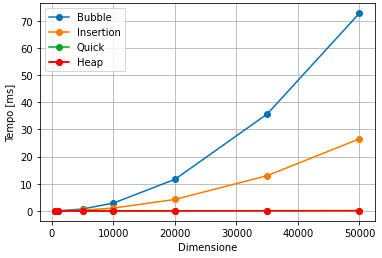
\includegraphics[width=\textwidth]{Img/GraficiSorting/Sorting1.png}
 \caption{Bubblesort insertionsort, heapsort e quicksort}
 \label{Fig:AllSortingAlg}
 \end{subfigure}
 \hfill
 \begin{subfigure}[t]{0.45\textwidth}
 \centering
 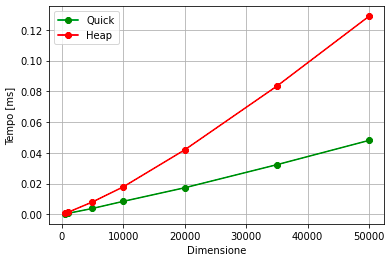
\includegraphics[width=\textwidth]{Img/GraficiSorting/Sorting2.png}
 \caption{Quicksort e Heapsort}
 \label{Fig:QHSort}
 \end{subfigure}

 \caption{Algoritmi di ordinamento a confronto}
 \label{Fig:AllSort}
\end{figure}


\subsection{Confronto Sorting}
In questa sezione vengono visualizzati i risultati a confronto. Per prima cosa iniziamo con confrontare i risultati con l'esecuzione su MacBook.


\begin{figure}[ht]
\centering
 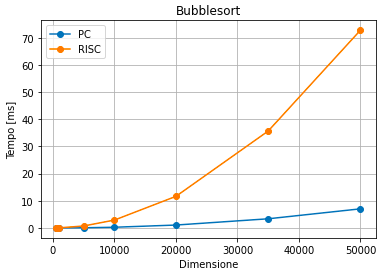
\includegraphics[scale=0.8]{Img/GraficiSorting/BubbleSort_Pc_Riscv.PNG}
 \caption{Tempi di esecuzione Bubblesort PC e RISC-V}
\end{figure}

\begin{figure}[ht]
\centering
 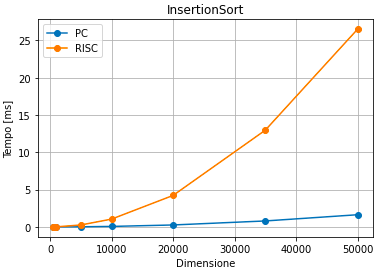
\includegraphics[scale=0.8]{Img/GraficiSorting/InsertionsortPcRisc.PNG}
 \caption{Tempi di esecuzione Insertionsort PC e RISC-V}
\end{figure}
	
\begin{figure}[ht]
\centering
 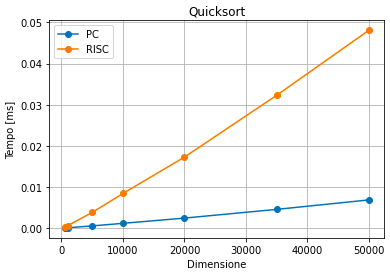
\includegraphics[scale=0.8]{Img/GraficiSorting/QuicksortPCRisc.PNG}
 \caption{Tempi di esecuzione Quicksort PC e RISC-V}
\end{figure}

\begin{figure}[ht]
\centering
 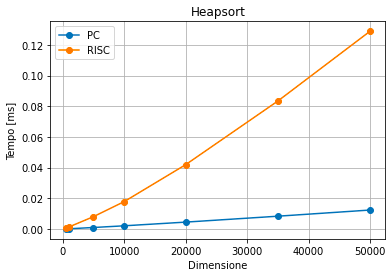
\includegraphics[scale=0.8]{Img/GraficiSorting/Heapsort_PC_RISC}
 \caption{Tempi di esecuzione Heapsort PC e RISC-V}
\end{figure}


	\begin{table}[ht]
		\centering
		\begin{tabular}		{| l | c | c | c | c |}
		\hline
		 & Bubblesort & Insertionsort & Heapsort & Quicksort \\ \hline
500 & 0.000491 & 0.000196 & 0.000057 & 0.000052 \\ \hline
1000 & 0.001871	 & 0.000723 & 0.000145 & 0.000080 \\ \hline
5000 & 0.055505 & 0.016859 & 0.000975 & 0.000544 \\ \hline
10000 & 0.247916 & 0.066411 & 0.002083 & 0.001164 \\ \hline
20000 & 1.056383 & 0.261627 & 0.004485 & 0.002441 \\ \hline
35000 & 3.359662 & 0.800075 & 0.008340 & ;0.004557 \\ \hline
50000 & 7.019640 & 1.633171 & 0.012359 & 0.006857 \\ \hline

		\end{tabular}
		\caption{Tempi di esecuzione degli algoritmi di sorting su PC in ms}
		\label{Fig:PcSort}
	\end{table}

La tabella \ref{Fig:PcSort} mostra i tempi di esecuzione degli algoritmi di ordinamento eseguiti sul PC. 
Un altro confronto lo possiamo fare con Raspberry pi \footnote{Il modello utilizzato è il modello Raspberry model B mostrato in figura \ref{fig:RaspberryB} }.



\begin{table}[ht]
		\centering
		\begin{tabular}		{| l | c | c | c | c |}
		\hline
		 & Bubblesort & Insertionsort & Heapsort & Quicksort \\ \hline
500 & 0.020337 & 0.004877 & 0.000825 & 0.000511 \\ \hline
1000 & 0.078527	 & 0.020353 & 0.001894 & 0.001141 \\ \hline
5000 & 2.030446 & 0.045018 & 0.013863 & 0.009072 \\ \hline
10000 & 8.535436 & 1.874295 & 0.027671 & 0.018542 \\ \hline
20000 & 34.733894 & 7.842624 & 0.058596 & 0.038194 \\ \hline
35000 & 117.622606 & 24.076289 & 0.114716 & 0.082891 \\ \hline
50000 & 250.008917 & 51.757841 & 0.210807 & 0.157344 \\ \hline

		\end{tabular}
		\caption{Tempi di esecuzione Raspberry Pi B in ms}
		\label{Tab:RaspSorting}
			\end{table}

\begin{figure}[ht]
\centering
	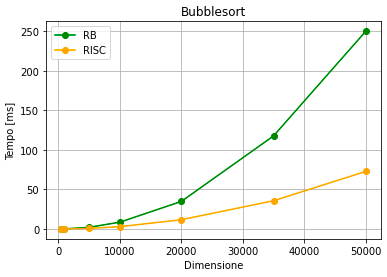
\includegraphics[scale=0.8]{Bubblesort_RB_RISC.PNG}
	\caption{Tempi di esecuzione Bubblesort Raspberry e RISC-V}
	\label{GrafBubble}
\end{figure}

\begin{figure}[ht]
\centering
	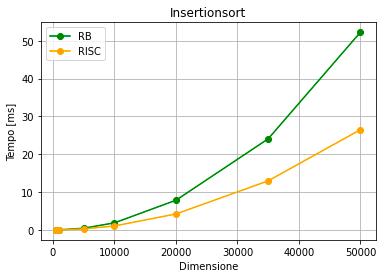
\includegraphics[scale=0.8]{Insertionsort_RB_RISC.PNG}
	\caption{Tempi di esecuzione Insertionsort Raspberry e RISC-V}
	\label{GrafInsertion}
\end{figure}
\begin{figure}[ht]
\centering
	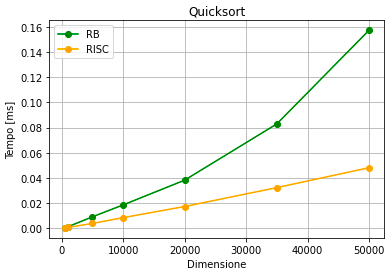
\includegraphics[scale=0.8]{Quicksort_RB_RISC.PNG}
	\caption{Tempi di esecuzione Quicksort Raspberry e RISC-V}
	\label{GrafQuick}
\end{figure}
\begin{figure}[ht]
\centering
	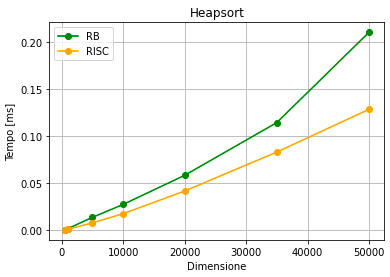
\includegraphics[scale=0.8]{Heapsort_RB_RISC.PNG}
	\caption{Tempi di esecuzione Heapsort Raspberry e RISC-V}
	\label{GrafHeap}
\end{figure}

I grafici \ref{GrafBubble} \ref{GrafInsertion} \ref{GrafQuick} \ref{GrafHeap} mostrano i tempi di esecuzione degli algoritmi di sorting comparati tra Rasberry e RISC-V. In ogni grafico si vede che il tempo di esecuzione è migliore su RISC-V. 
La tabella \ref{Tab:confrontoPrestazioniSorting} mostra il rapporto tra gli algoritmi eseguiti sul Raspberry e quelli eseguiti sulla board RISC-V. Prendendo in considerazione il Bubblesort nel caso con 50000 elementi, la board con processore RISC-V è 3.44 volte pi\'u veloce del raspberry in altri casi, come ad esempio per heap sort, il miglioramente di RISC-V è 1.64 rispetto a Raspberry. In media abbiamo un miglioramento di 2.12.Il che significa che la board in esame esegue il doppio pi\'u velocemente gli algoritmi di ordinamento del Raspberry.


\begin{figure}[ht]
\centering
 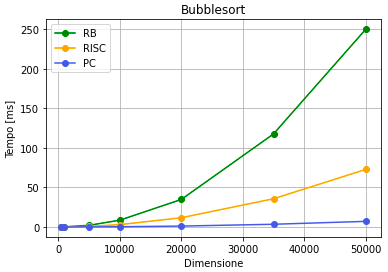
\includegraphics[scale=0.8]{Img/GraficiSorting/Bubblesort_All.PNG}
 \caption{Tempi di esecuzione Bubblesort}
\end{figure}

\begin{figure}[ht]
\centering
 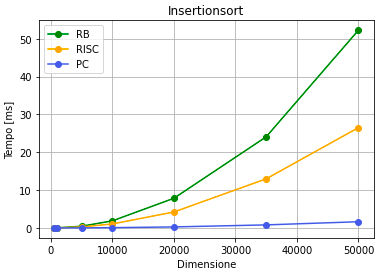
\includegraphics[scale=0.8]{Img/GraficiSorting/Insertionsort_All.PNG}
 \caption{Tempi di esecuzione Insertionsort}
\end{figure}
	
\begin{figure}[ht]
\centering
 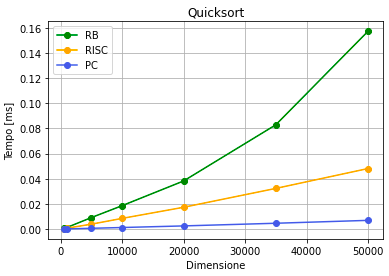
\includegraphics[scale=0.8]{Img/GraficiSorting/Quicksort_All.PNG}
 \caption{Tempi di esecuzione Quicksort}
\end{figure}

\begin{figure}[ht]
\centering
 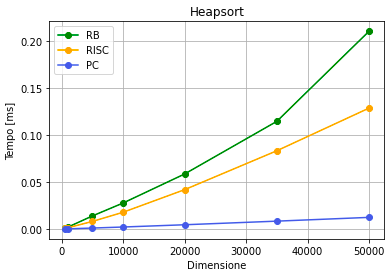
\includegraphics[scale=0.8]{Img/GraficiSorting/Heapsort_All}
 \caption{Tempi di esecuzione Heapsort}
\end{figure}


\begin{table}[ht]
\centering
\begin{tabular}{|l|l|l|l|l|l|}
\hline
      & Bubblesort & Insertionsort & Heapsort & Quicksort &      \\ \hline
500   & 2.84       & 1.85          & 1.45     & 1.87      &      \\ \hline
1000  & 2.73       & 1.92          & 1.49     & 1.87      &      \\ \hline
5000  & 2.83       & 0.17          & 1.73     & 2.38      &      \\ \hline
10000 & 2.95       & 1.79          & 1.55     & 2.20      &      \\ \hline
20000 & 2.99       & 1.86          & 1.40     & 2.21      &      \\ \hline
35000 & 3.30       & 1.86          & 1.38     & 2.57      &      \\ \hline
50000 & 3.44       & 1.95          & 1.64     & 3.27      &      \\ \hline
Media & 3.01       & 1.63          & 1.52     & 2.34      & 2.12 \\ \hline
\end{tabular}
\caption{Rapporto prestazioni RISC-V e ARM}
\label{Tab:confrontoPrestazioniSorting}
\end{table}


%--------

\chapter{Conclusione}
%PUNTI conclusivi(cosa posso dire)
% ISA -> due parole per sottolineare open
% Risultati CoreMark
% Risultati linpack
% Codice comparato: RISC-V piu linee di codice che ARM
% commentare

%ISA
In questa tesi si sono fatti alcuni test su RISC-V. 

%CoreMark, Linpack

%Multshift
Per quanto riguarda il codice assembly, generato il compilatore RISC-V genera codici di dimensioni maggiori rispetto ad ARM. RISC-V richiede pi\'u spazio quindi è pi\'u costoso in termini di memoria di programma richiesta, ma richiede meno cicli di clock per esecuzione. I codici riportati mostrano che la media richiesta da ARM \'e di 2.03 CPI mentre per RISC-V \'e 1.34. Il che significa che in media una singola istruzione per ARM richiede circa due cicli per essere completata mentre RISC-V per una singola istruzione, in media, richiede meno di due cicli. Inoltre, grazie alla sua struttura RISC-V ha un numero maggiore di Istruzioni per clock (IPC). 
%I processore RISC-V richiedono un numero di clock per l'esecuzione minore rispetto ai processori ARM e, grazie alla struttura e all'ISA, hanno un numeri di istruzioni per ciclo minori rispetto a RISC-V. 

%Sorting
Per quanto riguarda il sorting, il confronto con gli algoritmi tra RISC-V, il Raspberry e il pc, mostra che la board dotata di RISC-V è sempre più veloce del Raspberry in ogni algoritmo ma è sempre più lento del pc. Rispetto ai tempi di esecuzione del Raspberry la board
migliora il tempo di esecuzione in media di 2.12. 
\todo{riassumi qualche numero, di quanto?}
\todo{mattia: aggiunto}
Possiamo concludere osservando che la board RISC-V è una valida sostituta del Raspberry in termini di velocit\'a di calcolo.% ma il codice che genera il compilatore RISC-V è di dimensione maggiore rispetto a quello di ARM.

%consumo di potenza %potenza per watt %area x costo
Utilizzando anche altri studi condotti su RISC-V fatte su consumi e potenza,
sempre comparando RISC-V con ARM, i processori RISC-V consumano meno potenza rispetto ad ARM e offrono prestazioni migliori per watt.  Per quanto riguarda i costi dei chip, i processori RISC-V tendono ad avere dimensioni inferiori rispetto ai processori ARM quindi meno costosi in termini di silicio, rendendoli più adatti per applicazioni sensibili ai costi \cite{blogArmRISC-V}.

In conclusione possiamo affermare che il progetto RISC-V, nato come progetto didattico, \'e arrivato sul mercato supportato da una community sempre pi\'u crescente che lo ha portato a notevoli sviluppi. Oggi si affaccia sul mercato affiancandosi con ARM dando la possibilit\'a ai progettisti di scegliere un'alternativa free e open-source per le loro necessit\'a. L'offerta di RISC-V \'e di una tecnologia a basso consumo, a costo ridotto di materiale, con la possiblit\'a di personalizzare liberamente l'ISA per specifiche funzionalit\'a. Con queste premesse le aree di applicazione della tecnologia RISC-V sono molteplici. 


Le aree di applicazione di RISC-V oggi sono i \textit{microcontrollers} e il mondo embedded dove vengono progettati piccoli dispositivi a basso consumo per svolgere determinate funzioni che possono essere per \textit{smart home} o dispositivi IoT.
Un altra area di applicazione \'e il \textit{machine learning} grazie alla loro configurabilità ottengono la possibilità di soddisfare requisiti specifici.
%Anche in ambito accademico 


Questa tesi analizza solo alcuni aspetti di RISC-V. 
Terminato questo lavoro di tesi vorrei sottolineare che non si tratta di un lavoro concluso, ma un punto di partenza per possibili approfondimenti futuri. 

\todo{conclusione minimale, riesci a dire se ci sono aspetti in cui uno è meglio dell'altro e viceversa? comparazioni di costo? corrente consumata? ecc.}
\todo{mattia: ok}

\todo{atrent: nelle conclusioni dovresti a questo punto (a valle del tuo lavoro di analisi) poter dire non solo come si confronta risc-v con gli altri, ma anche quali sono le aree di debolezza e forza, tanto da ipotizzare quale potrebbero essere i contesti d'uso favorevoli}
\todo{mattia: ok?}

%\addcontentsline{toc}{chapter}{Bibliografia}

\printbibliography 

\end{document}
